\documentclass[12pt]{article}
\usepackage{tabularx}
\usepackage{multirow}
\usepackage{makecell}
\usepackage{changepage}
\usepackage{xifthen}
\usepackage{amsmath}
\usepackage{amssymb}
\usepackage{setspace}
\usepackage{xcolor}
\usepackage{graphicx,caption}
\usepackage{subcaption}
\usepackage{enumitem}
\usepackage{caption}
\usepackage{array}
\usepackage{booktabs}
\usepackage{hyperref}
\hypersetup{colorlinks=true,linkcolor=blue}
\usepackage{comment}
\usepackage[backend=biber]{biblatex}
\addbibresource{ref.bib}

\parindent 0em
\setcounter{secnumdepth}{3}
\setcounter{tocdepth}{3}

\renewcommand{\baselinestretch}{1.2}
\usepackage[includehead,left=3.25cm,right=2.5cm,top=2.5cm,headsep=1.5cm,headheight=0.0cm,bottom=2.5cm,footskip=1.0cm]{geometry}
\raggedbottom

\title{\textbf{Channel-Aware Cooperative Perception for Blind Spot Detection in V2X Networks}}

\author{Aiden McGarrie, Rageshwaree Beegodhur, Vanessa Vo \\ \textit{School of Electrical Engineering and Computer Science,} \\ \textit{University of Ottawa, Canada}}

\date{}

\begin{document}

\maketitle

\begin{abstract}
\noindent
Autonomous vehicles have become a focal point of research and development because of their ability to perceive their surroundings. However, physical obstructions and limited perceptions create blind spots onboard sensors cannot resolve alone. This report proposes a channel-aware cooperative vehicle-infrastructure perception system that addresses this issue by using a Roadside Unit (RSU) to detect objects in blind spots and selectively transmit the information to nearby vehicles using a bandwidth-constrained Vehicle-to-Everything (V2X) channel.

\medskip
\noindent
The system operates as an end-to-end pipeline on the DAIR-V2X dataset, combining YOLOv10-N object detection, ByteTrack multi-object tracking, and bird's eye view localization using monocular depth and LiDAR calibration. A Hungarian matching algorithm with a depth-aware Mahalanobis distance cost matrix identifies blind spot targets, and a lightweight Multi-Layer Perceptron (MLP) Semantic Gate prioritizes which targets to transmit under realistic per-frame bandwidth budgets.

\medskip
\noindent
Comparative testing demonstrates the MLP Semantic Gate consistently outperforms Hard Gate, No Gate, and Random baselines across all transmission levels, achieving a precision-recall score of 0.551 compared to a random baseline of 0.023. The results highlight that prioritizing bandwidth meaningfully improves cooperative perception under real-world communication constraints.
\end{abstract}

\newpage
\tableofcontents
\newpage

\section{Introduction}
Cars driving through busy intersections can only see what their sensors can reach. Objects such as buildings, trucks, other cars consistently block the sensors view, creating blind spots that can lead to accidents. This issue can not just be fixed by adding more sensors to the car because something will always remain hidden. 

\medskip
A practical answer to this problem is to integrate RSUs, cameras and sensors mounted at intersections because they are able to scan the environment transmit the information to nearby vehicles, preventing collisions. 

\medskip
The challenge of cooperative perception is not scanning the surroundings, but the communication between the RSUs and the vehicles. An RSU might detect up to fourty objects in a busy intersection per frame but the V2X channel has limited bandwich, meaning that the RSU cannot send everything. What the RSU decides to transmit can not be random and must consider what the vehicle already knows to maximize the amount of channel bandwidth used to fill the vehicle's blind spots. Thus, the question is how to find what objects are in the vehicle's blind spot and how to determine which ones are worth sending. 

\medskip
This paper describes a system created to answer that question. Using the DAIR-V2X dataset \cite{yu2022dairv2x}, we built a full pipeline that runs detection using YOLOv10-N \cite{wang2024yolov10}, tracks objects over time with ByteTrack \cite{zhang2022bytetrack}, converts detections into shared world coordinates, matches RSU and vehicle object lists to find what the vehicle is missing, and then uses a trained MLP to decide what is worth transmitting given the available bandwidth. Then, the matching step uses Mahalanobis distance rather than simple Euclidean distance, which matters because position uncertainty grows with depth and a naive distance metric ignores that entirely.

\medskip
The contributions of this work are:
\begin{itemize}
    \item A complete cooperative perception pipeline running on real DAIR-V2X data, from raw frames to identified blind spot targets.
    \item A depth-aware covariance model for bird's eye view matching that accounts for how uncertainty scales with distance.
    \item A channel-aware MLP Semantic Gate trained to prioritize true blind spot targets under five different bandwidth levels (L0--L4).
    \item An evaluation comparing MLP, Hard Gate, No Gate, and Random strategies using mAP at 2m, 4m, and 6m thresholds, alongside recall and precision-recall metrics.
\end{itemize}

\section{Related Work}
\label{sec:related}

\subsection{Cooperative Perception and V2X Communication}

Sharing data between vehicles is not a new idea. V2VNet \cite{wang2020v2vnet} was one of the first to share feature maps between vehicles but assumed unlimited bandwidth would be unrealistic. 
\medskip
Where2comm \cite{hu2022where2comm} used spatial confidence maps to seperate only the important parts of the scence, transmitting only those parts, which significantly cut down volume while preserving accuracy.  Newer work goes begins to explore what features are actually useful for the task. Our pipeline uses similar logic, and scores every blind spot candidate by how relevent it is to the vehicle of interest and only traansmits the highest ranking ones. 

\subsection{Object Detection}

Object detection is used to find and classify objects in images and there are two main types: two-stage and single-stage detectors. Faster R-CNN \cite{ren2016faster} is a two-stage detector that proposes candidate regions first and classifies them after. This apporach results in strong accuracy but is slow, which makes it difficult to use in real-world scenarios. Alternatively, single-stage detectors like the You Only Look Once (YOLO) \cite{redmon2016yolo}, does everything in one pass, which slightly decreased the overall accuracy for a large increase in speed.

\medskip
YOLOv10 \cite{wang2024yolov10} is the detection model used in this work. It removes the need for non-maximum suppression at inference time by using a dual-label assignment strategy during training, which simplifies the pipeline and improves end-to-end speed. The Nano variant, YOLOv10-N, is the smallest member of the family and is specifically intended for hardware with limited compute which is a realistic constraint for an RSU running at the edge.

\subsection{Multi-Object Tracking}

Only using detection outputs boxes pper frame but does not have memory across time.. Tracking connects those boxes into trajectories, assigning consistent identities so that the same vehicle keeps the same ID across hundreds of frames. ByteTrack \cite{zhang2022bytetrack}  can do this by matching low-confidence and high-confidence detections when previously, low-confidence detections were discarded. The reasoning is straightforward: a partially occluded vehicle may generate a weak detection, but it is still the same vehicle and losing track of it causes problems downstream. ByteTrack's ability to match both high and low-confidence detectionsreduces the number of identity switches in high traffic frames which is vital for maintaining stable tracks that can be projected intoo world coordinates and matched across views.

\subsection{Probabilistic Matching and Mahalanobis Distance}

When a camera detection is projected into world coordinates, a single point is not returned, but a distribution that grows in size as distance increases. This is because the monocular depth estimation error increases with distance, and the error is not symetrical: the uncertainty is not equal in all directions, the depth error increases much faster than lateral error. A matching algorithm that treats each detection as a precise point and measures Euclidean distance between them ignores all of this, leading to false matches at range and missed matches near the camera where everything is crowded together.

\medskip
The Mahalanobis distance \cite{mahalanobis1936} addresses this by folding the covariance structure of each detection's uncertainty directly into the distance calculation. Two detections that are far apart in meters but within each other's uncertainty ellipses will have a small Mahalanobis distance; two detections that are close in meters but with very different uncertainty structures will have a larger one. Paired with the Hungarian algorithm \cite{kuhn1955hungarian} for optimal one-to-one assignment, this gives a matching framework that is substantially more robust to the noise inherent in real-world BEV projections.

\section{Methodology}
\label{sec:method}

\subsection{Dataset}

All experiments in this paper use the DAIR-V2X Cooperative dataset \cite{yu2022dairv2x}, recorded in urban China across a range of real intersection scenarios. The dataset pairs a vehicle-mounted camera with a fixed infrastructure RSU camera at the same location, providing synchronized frames from both viewpoints along with LiDAR scans, 3D bounding box annotations, and full sensor calibration for both platforms.

\medskip
There are 8,577 vehicle-side frames and 15,285 infrastructure-side frames in total. Each frame comes with ground-truth 3D labels giving the true world position of every object in the scene, which we use both to generate training labels for the Semantic Gate and to evaluate blind spot detection accuracy at the end. The calibration files provide the extrinsic and intrinsic parameters needed to move detections out of image space and into a shared world coordinate system. Without these, cross-view matching would not be possible.

\medskip
Seven classes are detected throughout: Car, Van, Bus, Truck, Cyclist, Motorcyclist, and Trafficcone. For training the vehicle-side detector we split the data 80/20 into 12,228 training images and 3,057 validation images, using a fixed random seed of 42 so the split is reproducible. DAIR-V2X stores labels as JSON files with pixel-coordinate bounding boxes in \texttt{(xmin, ymin, xmax, ymax)} format; these were converted to YOLO's normalized \texttt{(class\_id, x\_center, y\_center, width, height)} format before training.

\subsection{System Pipeline Overview}

The pipeline runs two streams in parallel: one processing RSU frames, one processing vehicle frames, and merges them at the matching stage. Figure~\ref{fig:pipeline} shows the full flow.

\begin{figure}[htbp]
\centering
\includegraphics[width=\textwidth]{pipeline_diagram.png}
\caption{System pipeline. Infrastructure and vehicle streams are processed independently through detection, tracking, and BEV localization before being fused at the Hungarian matching stage to identify blind spot targets, which are then ranked by the Semantic Gate MLP for transmission.}
\label{fig:pipeline}
\end{figure}

\medskip
Both streams start with YOLOv10-N producing per-frame detections. ByteTrack then links those detections into tracks with stable IDs. The tracked detections are lifted out of image space into bird's eye view world coordinates using monocular depth and LiDAR calibration data. At the fusion point, the Hungarian algorithm with a Mahalanobis cost matrix matches RSU objects to vehicle objects and anything on the RSU side with no match on the vehicle side is flagged as a blind spot candidate. The Semantic Gate MLP then scores each candidate and selects the top-N to transmit, where N comes from the simulated channel budget.

\subsection{Object Detection Training}

YOLOv10-N was chosen as the detector for both streams. The decision came down to speed and size: as the smallest variant in the YOLOv10 family, it is built for edge deployment on limited hardware, which is a realistic constraint for an RSU running at an intersection. Separate models were trained for the vehicle-side and infrastructure-side cameras since the viewing angles and object appearance differ substantially between the two.

\medskip
\textbf{Training setup.} The vehicle-side model was trained for 150 epochs on an RTX 3070 GPU, taking roughly 8.3 hours. Input resolution was 640$\times$640 with a batch size of 16. We used SGD with a cosine learning rate schedule and standard YOLO data augmentation.

\medskip
\textbf{Results.} Figure~\ref{fig:training_curves} shows the training and validation curves over all 150 epochs. Loss drops consistently across all three components: box, classification, and distribution focal loss on both train and validation sets. There is no visible gap opening between the two, which suggests the model is not overfitting. Precision and recall climb steadily and plateau near the end of training.

\begin{figure}[htbp]
\centering
\includegraphics[width=\textwidth]{results.png}
\caption{Training and validation loss curves and validation metrics over 150 epochs for the vehicle-side YOLOv10-N model.}
\label{fig:training_curves}
\end{figure}

\medskip
Final validation metrics at epoch 150 are shown in Table~\ref{tab:detection_results}. The model reaches a precision of 0.828 and recall of 0.663, with mAP@50 of 0.737 and mAP@50-95 of 0.475.

\begin{table}[htbp]
\centering
\caption{Vehicle-side YOLOv10-N validation results at epoch 150.}
\label{tab:detection_results}
\begin{tabular}{lcccc}
\toprule
\textbf{Model} & \textbf{Precision} & \textbf{Recall} & \textbf{mAP@50} & \textbf{mAP@50-95} \\
\midrule
YOLOv10-N (vehicle-side) & 0.828 & 0.663 & 0.737 & 0.475 \\
\bottomrule
\end{tabular}
\end{table}

\medskip
Per-class performance is visible in the Precision-Recall curve in Figure~\ref{fig:pr_curve}. Bus comes out on top at mAP@50 of 0.901, followed by Car at 0.850 and Truck at 0.842. Trafficcone is the weakest at 0.407 because it is small, often partially occluded, and appears far less frequently than cars in the training data, which all work against it. Cyclist and Motorcyclist sit in the middle at 0.669 and 0.703 respectively, reflecting the challenge of detecting smaller, more articulated objects from a forward-facing vehicle camera.

\begin{figure}[htbp]
\centering
\includegraphics[width=0.75\textwidth]{BoxPR_curve.png}
\caption{Per-class Precision-Recall curves. The bold blue line shows overall mAP@50 of 0.737.}
\label{fig:pr_curve}
\end{figure}

\medskip
The F1-Confidence curve in Figure~\ref{fig:f1_curve} peaks at 0.73 across all classes at a confidence threshold of 0.301. Bus and Truck lead here too, consistent with their stronger mAP scores. The fact that the peak sits at a fairly low confidence threshold reflects the dataset's difficulty. Pushing confidence higher cuts recall faster than it improves precision for most classes.

\begin{figure}[htbp]
\centering
\includegraphics[width=0.75\textwidth]{BoxF1_curve.png}
\caption{F1-Confidence curves per class. Peak all-classes F1 of 0.73 at confidence threshold 0.301.}
\label{fig:f1_curve}
\end{figure}

\medskip
Figure~\ref{fig:confusion} shows the normalized confusion matrix. Bus (0.87) and Car (0.81) are classified most reliably. The main confusion patterns make intuitive sense: 13\% of Cars are called Vans, and 5\% of Motorcyclists are called Cyclists. These pairs look similar from a front-facing camera, particularly at distance. Trafficcone has the worst background confusion rate at 0.62, meaning the model misses it outright most of the time. This is a known challenge with small, thin objects in complex backgrounds.

\begin{figure}[htbp]
\centering
\includegraphics[width=0.75\textwidth]{confusion_matrix_normalized.png}
\caption{Normalized confusion matrix for the vehicle-side YOLOv10-N model on the validation set.}
\label{fig:confusion}
\end{figure}

\medskip
Figure~\ref{fig:val_predictions} shows a sample validation batch with ground truth on the left and model predictions on the right. The model correctly localizes the dominant classes across a range of urban scenes, with the main visible errors occurring on distant or partially occluded objects.

\begin{figure}[htbp]
\centering
\begin{subfigure}[b]{0.48\textwidth}
    \includegraphics[width=\textwidth]{val_batch0_labels.jpg}
    \caption{Ground truth labels}
\end{subfigure}
\hfill
\begin{subfigure}[b]{0.48\textwidth}
    \includegraphics[width=\textwidth]{val_batch0_pred.jpg}
    \caption{Model predictions}
\end{subfigure}
\caption{Validation batch: ground truth (left) vs YOLOv10-N predictions (right) on vehicle-side DAIR-V2X images.}
\label{fig:val_predictions}
\end{figure}

% -----------------------------------------------
% PERSON B SECTIONS GO HERE
% 3.4 BEV Coordinate System & LiDAR Projection
% 3.5 ByteTrack Integration
% 3.6.1 Hungarian Matching
% 4.1 Experiment Setup
% 4.2 Strategy Comparison
% 4.4 Transmission Level Comparison
% -----------------------------------------------

% -----------------------------------------------
% PERSON C SECTIONS GO HERE
% 3.6.2 Mahalanobis Distance & Covariance Model
% 3.6.3 Covariance Parameter Calibration
% 3.7 Semantic Gate MLP
% -----------------------------------------------
\subsection{Mahalanobis Distance and Covariance Model}
\label{sec:mahalanobis}

A fixed Euclidean threshold treats every detection as equally certain regardless of how far away it is or which sensor produced it. That assumption breaks in practice. Monocular depth estimates grow less accurate with distance, and that error is not symmetric: longitudinal uncertainty (depth) grows much faster than lateral uncertainty. Using a single distance threshold means the gate is too tight for distant objects, causing missed matches, and too loose for nearby ones, causing false matches.

\medskip
The Mahalanobis distance~\cite{mahalanobis1936} folds each detection's positional covariance directly into the cost matrix. Given two objects $a$ and $b$ with world-coordinate centers $\mathbf{p}_a, \mathbf{p}_b \in \mathbb{R}^2$ and covariances $\Sigma_a, \Sigma_b \in \mathbb{R}^{2\times 2}$, the distance is

\begin{equation}
    d_M(a,b) = \sqrt{(\mathbf{p}_a - \mathbf{p}_b)^\top
               \bigl(\Sigma_a + \Sigma_b + \varepsilon\mathbf{I}\bigr)^{-1}
               (\mathbf{p}_a - \mathbf{p}_b)},
    \label{eq:mahalanobis}
\end{equation}

\noindent where $\varepsilon = 10^{-3}$ is a regularization term that keeps the combined covariance invertible. The combined covariance $\Sigma_a + \Sigma_b$ widens the gate for uncertain detections and tightens it where both estimates are reliable.

\medskip
Each object's covariance is constructed from its camera-frame depth $Z_c$ and the rotation $R \in \mathbb{R}^{2\times 2}$ mapping camera BEV axes $(X_c, Z_c)$ to world BEV axes $(X_w, Y_w)$. The camera-frame covariance is diagonal:

\begin{equation}
    \Sigma_{\text{cam}}(Z_c) =
    \begin{pmatrix} \sigma_x^2 & 0 \\ 0 & \sigma_z^2 \end{pmatrix},
    \label{eq:cov_cam}
\end{equation}

\noindent with lateral spread $\sigma_x = \max(\sigma_{x_0} + k_x Z_c,\;\sigma_{\text{floor}})$ growing linearly with depth, and longitudinal spread $\sigma_z = \max(k Z_c^2,\;\sigma_{\text{floor}})$ growing quadratically, matching the known behavior of monocular depth error. A floor $\sigma_{\text{floor}}$ prevents the covariance from collapsing to zero at very short range.

\medskip
The world-frame covariance is obtained by rotating through the BEV projection:

\begin{equation}
    \Sigma_{\text{world}}(Z_c, R) = R\,\Sigma_{\text{cam}}(Z_c)\,R^\top,
    \label{eq:cov_world}
\end{equation}

\noindent where $R$ is extracted from the LiDAR-to-world and LiDAR-to-camera rotation matrices as

\begin{equation}
    R_{\text{bev}} = \bigl(R_{l2w} \cdot R_{l2c}^\top\bigr)_{[\{0,1\},\{0,2\}]}.
\end{equation}

\noindent The subscript selects the two rows and two columns that project from the camera's $(X_c, Z_c)$ plane into the world's $(X_w, Y_w)$ plane. When depth or calibration data are unavailable, the covariance falls back to $\sigma_{\text{fallback}}^2\mathbf{I}$ with $\sigma_{\text{fallback}} = 3.0$\,m, creating a loose gate that avoids false rejections under degraded inputs.

\medskip
The Mahalanobis cost matrix is built over all $N_r \times N_v$ roadside and vehicle-side candidate pairs. A gate threshold derived from the chi-squared distribution,

\begin{equation}
    d_{\text{thresh}} = \sqrt{\chi^2_{0.99,\,df=2}} \approx 3.035,
\end{equation}

\noindent corresponds to the 99\% confidence ellipse of the joint 2-D Gaussian. Pairs exceeding $3\times d_{\text{thresh}}$ are assigned a large cost $c_{\text{large}} = 10^6$ before the Hungarian solver~\cite{kuhn1955hungarian} runs, preventing implausible assignments from distorting the overall solution. After assignment, only pairs with $d_M < d_{\text{thresh}}$ are accepted as true matches; all others become unmatched blind spot candidates. Class labels are additionally enforced: a roadside Car will not be matched to a vehicle-side Truck regardless of spatial proximity.

\subsection{Covariance Parameter Calibration}
\label{sec:calibration}

The three parameters $k$, $\sigma_{x_0}$, and $k_x$ of the covariance model need to reflect how much error the system actually makes at different depths, rather than being chosen by hand. We calibrate them from ground-truth-matched object pairs when sufficient data are available and fall back to conservative defaults otherwise.

\medskip
The procedure works as follows. For each matched pair we compute the world-frame residuals

\begin{equation}
    \varepsilon_x = X_w^{\text{pred}} - X_w^{\text{gt}}, \qquad
    \varepsilon_r = \sqrt{\varepsilon_x^2 + \varepsilon_y^2},
\end{equation}

\noindent bin the errors by depth into $[0,20),\;[20,40),\;[40,60),\;[60,120)$\,m intervals, and compute empirical standard deviations $\hat{\sigma}_x$ and $\hat{\sigma}_r$ per bin (bins with fewer than 10 samples are discarded). The quadratic parameter $k$ is then fitted by no-intercept least squares:

\begin{equation}
    k = \frac{\sum_i \hat{\sigma}_{r,i}\,Z_i^2}{\sum_i Z_i^4},
\end{equation}

\noindent and the lateral parameters $\sigma_{x_0}$, $k_x$ are estimated by ordinary least squares on $\hat{\sigma}_{x,i} = \sigma_{x_0} + k_x Z_i$.

\medskip
On the DAIR-V2X cooperative split, 364 of the 462 frames containing blind spot candidates produced no ground-truth matches within the 50\,m search radius, suggesting calibration or synchronization inconsistencies between the infrastructure and vehicle world frames. The remaining 98 frames yielded supervision at the object level: 14{,}644 candidate objects in total, of which 348 (2.4\%) were confirmed positives. Training operates on these object-level labels rather than frame-level counts, so the effective supervised set is 348 positive and 14{,}296 negative objects across those 98 frames. When the matched dataset contains fewer than two valid depth bins, the system falls back to default parameters $(k=0.01,\;\sigma_{x_0}=0.3\,\text{m},\;k_x=0.005)$, which represent conservative uncertainty bounds for automotive-scale scenes and were used in the experiments reported below.

\subsection{Semantic Gate MLP}
\label{sec:semantic_gate}

The Hungarian matching step produces a list of blind spot candidates: infrastructure detections that have no match on the vehicle side. On this dataset, that list averages $31.7 \pm 18.3$ candidates per frame. Transmitting all of them is not feasible because the V2X channel budget can drop to single-digit objects per frame at higher transmission levels. The Semantic Gate ranks candidates by priority and selects the top $N_{\max}$ for transmission, where $N_{\max}$ is set by the channel at runtime.

\subsubsection{Architecture and Feature Design}
\label{sec:gate_arch}

The gate is implemented as a three-layer MLP with 3{,}201 total parameters:

\begin{equation}
    \hat{s} = \sigma\!\left(
        W_3\;\text{ReLU}\!\left(
            W_2\;\text{ReLU}\!\left(W_1\,\mathbf{f} + b_1\right) + b_2
        \right) + b_3
    \right),
\end{equation}

\noindent where $W_1 \in \mathbb{R}^{64\times 16}$, $W_2 \in \mathbb{R}^{32\times 64}$, $W_3 \in \mathbb{R}^{1\times 32}$, $\sigma$ is the sigmoid function, and dropout ($p=0.2$) follows each hidden layer during training. The output $\hat{s} \in [0,1]$ is the transmission priority score for a single candidate.

\medskip
Each candidate is described by a 16-dimensional feature vector $\mathbf{f}$ built as follows:

\begin{itemize}[noitemsep]
    \item \textbf{Dims 0--6:} One-hot class encoding (Car, Van, Cyclist, Motorcyclist, Trafficcone, Bus, Truck).
    \item \textbf{Dim 7:} YOLO detection confidence score.
    \item \textbf{Dim 8:} Distance from the ego vehicle, normalized by 500\,m.
    \item \textbf{Dim 9:} Binary flag indicating whether the candidate lies within the ego vehicle's forward 120-degree sector. Of the 14{,}644 candidates, 8{,}439 (57.6\%) fall within this cone, and 193 of the 348 confirmed positives are also forward-facing.
    \item \textbf{Dims 10--11:} Ego-relative position $(x, y)$ rotated into the ego heading frame and normalized by 500\,m, making the representation invariant to absolute world coordinates.
    \item \textbf{Dim 12:} Total blind spot candidates in the current frame, normalized by 50 (mean $31.7$ per frame).
    \item \textbf{Dim 13:} Forward-sector candidates in the current frame, normalized by 50.
    \item \textbf{Dim 14:} Normalized channel capacity $C_{\text{norm}}$, injected at runtime.
    \item \textbf{Dim 15:} Budget ratio $\min(N_{\max}/n_{\text{cand}},\;1.0)$, the fraction of candidates that can actually be transmitted given the current channel state.
\end{itemize}

Dims 14 and 15 are not fixed at training time. They are injected fresh at each inference call so that a single trained model adapts its selection behavior to whatever channel conditions exist at the moment, without retraining.

\medskip
The forward sector flag (dim 9) encodes a geometric safety prior. Its membership test is

\begin{equation}
    \Delta\theta =
    \Bigl|\operatorname{atan2}(y_t - y_e,\;x_t - x_e) - \psi\Bigr|_{\pi},
\end{equation}

\noindent where $|\cdot|_\pi$ wraps to $[-\pi,\pi]$ and $\psi$ is the ego heading. A candidate qualifies if $\Delta\theta \leq 60^\circ$.

\medskip
Ground-truth labels are assigned by matching each candidate to the cooperative \texttt{label\_world} annotations using a 10\,m Hungarian match. A candidate is labeled $y=1$ if a ground-truth object falls within that radius, $y=0$ otherwise. The result is a heavily imbalanced dataset: 348 positives against 14{,}296 negatives, a 2.4\% positive rate.

\subsubsection{Training Procedure}

The dataset is split 80/20 at the frame level, giving 369 training frames (11{,}735 samples, 279 positives) and 93 validation frames (2{,}909 samples, 69 positives). Frame-level splitting prevents temporal leakage between the two sets.

\medskip
The loss combines Binary Cross-Entropy with Logits at positive class weight $w_+ = 51.5$ with a bandwidth penalty:

\begin{equation}
    \mathcal{L} = \mathcal{L}_{\text{BCE}} + \lambda_{\text{BW}}\,\mathcal{L}_{\text{BW}},
    \label{eq:total_loss}
\end{equation}

\noindent where the bandwidth penalty is a hinge on the total predicted score mass relative to the frame budget:

\begin{equation}
    \mathcal{L}_{\text{BW}} = \frac{1}{|\mathcal{B}|}
    \max\!\left(\sum_{i \in \mathcal{B}} \hat{s}_i - B_{\text{batch}},\;0\right),
    \label{eq:bw_loss}
\end{equation}

\noindent $B_{\text{batch}} = N_{\max} \times n_{\text{frames}}$ is the transmission budget for the batch, and $\lambda_{\text{BW}} = 0.1$. Without this term the model can inflate all scores uniformly and maximize recall trivially by always recommending everything. The hinge activates only when the total score mass exceeds the budget, penalizing that excess directly.

\medskip
Training uses Adam at $\eta = 5\times10^{-4}$ with gradient clipping at norm 1.0. At each batch a random channel condition $(C_{\text{norm}}, N_{\max})$ is sampled from the channel simulator (Section~\ref{sec:channel}) so the model sees a range of bandwidth regimes during training rather than just the conditions found in the dataset. Early stopping with patience 150 on validation recall terminated training at epoch 306, with the best checkpoint saved at epoch 156 (validation recall 0.609).

\medskip
The MLP is compared against three non-learned baselines under the same channel budget:
\begin{itemize}[noitemsep]
    \item \textbf{Hard Gate:} $s = 0.5\,\text{conf} + 0.3\,\text{is\_forward} + 0.2\,(1-d_{\text{norm}})$.
    \item \textbf{Random:} Candidates selected uniformly at random up to $N_{\max}$.
    \item \textbf{No Gate:} The first $N_{\max}$ candidates in arbitrary frame order.
\end{itemize}

\subsubsection{Channel Simulation}
\label{sec:channel}

The channel simulator computes $N_{\max}$ for each frame based on a log-distance path loss model with separate LOS and NLOS exponents:

\begin{equation}
    PL(d) = PL_0 + 10\,\alpha\,\log_{10}\!\left(\frac{d}{d_0}\right) + X_\sigma,
\end{equation}

\noindent where $PL_0 = 38$\,dB at reference distance $d_0 = 1$\,m, $\alpha \in \{2.0,\;3.5\}$ for LOS and NLOS respectively, and $X_\sigma \sim \mathcal{N}(0,\sigma_{\text{shadow}}^2)$ is log-normal shadowing. Rayleigh fading scaled by ego velocity models Doppler spread. Available capacity after subtracting background V2X traffic is

\begin{equation}
    C_{\text{avail}} = \max\!\left(
        \eta_{\text{MAC}} \cdot B\log_2(1 + \text{SNR}) - L_{\text{BG}},\;0
    \right),
\end{equation}

\noindent where $\eta_{\text{MAC}} = 0.4$ and $B = 10$\,MHz. The per-frame object budget is

\begin{equation}
    N_{\max} = \left\lfloor
        \frac{C_{\text{avail}} \cdot \Delta t}{8\,s_{\text{level}}}
    \right\rfloor,
\end{equation}

\noindent with $\Delta t = 0.1$\,s. The five transmission levels are defined in Table~\ref{tab:tx_levels}, alongside representative $N_{\max}$ values under two canonical scenarios. At L3 and L4 the budget drops to single digits even at short range with favourable LOS conditions, making intelligent selection essential. Figure~\ref{fig:channel} illustrates the resulting Shannon capacity curves and implied $N_{\max}$ across levels as a function of distance.

\begin{table}[h]
\centering
\caption{Transmission levels and $N_{\max}$ under Near/LOS (80\,m, SNR 53.9\,dB)
         and Medium/NLOS (200\,m, SNR 11.5\,dB) conditions.}
\label{tab:tx_levels}
\resizebox{\textwidth}{!}{%
\begin{tabular}{llrcc}
\toprule
\textbf{Level} & \textbf{Content} & \textbf{Size (B)}
    & \textbf{$N_{\max}$ Near/LOS}
    & \textbf{$N_{\max}$ Med./NLOS} \\
\midrule
L0 & Position, class, confidence, velocity        &     50 & 17{,}878 & 3{,}788 \\
L1 & L0 + motion history + uncertainty            &    256 &  3{,}491 &   739   \\
L2 & L1 + small BEV patch (8$\times$8$\times$16) & 2{,}048 &    436 &    92   \\
L3 & L2 + ROI crop (32$\times$32$\times$25)       & 51{,}200 &   17 &     3   \\
L4 & L3 + compressed feature map region           &204{,}800 &    4 &     1   \\
\bottomrule
\end{tabular}%
}
\end{table}

\begin{figure}[h]
\centering
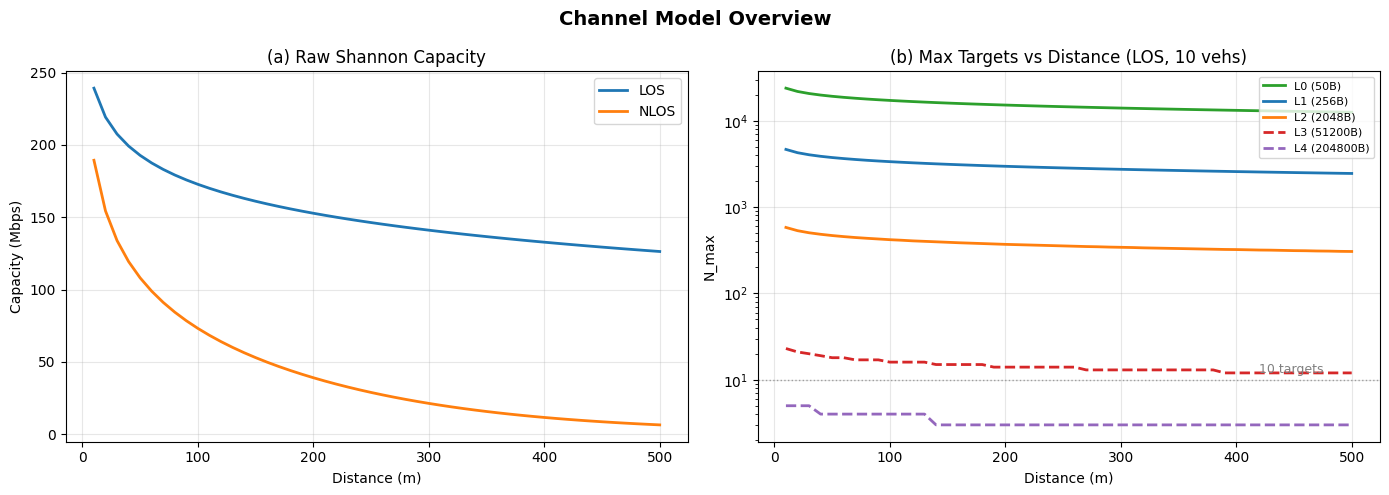
\includegraphics[width=\textwidth]{capacity_vs_distance.png}
\caption{Channel model overview. Left: raw Shannon capacity for LOS and NLOS
         path loss models. Right: maximum transmissible objects per frame ($N_{\max}$)
         across the five transmission levels as a function of ego-RSU distance under
         LOS conditions with 10 background vehicles. L3 and L4 (dashed) fall below
         10 targets per frame beyond 50\,m, motivating intelligent candidate selection.}
\label{fig:channel}
\end{figure}

\noindent LOS status per frame is determined geometrically using the Liang-Barsky algorithm in the BEV plane, checking whether any detected vehicle bounding box intersects the RSU-to-ego line of sight. The simulator was validated on 9{,}069 DAIR-V2X frame pairs, reporting a mean $C_{\text{norm}}$ of 0.624 at L0 and mean SNR of 36.8\,dB. The full dataset shows 100\% LOS classification and a mean ego-RSU distance of 1{,}059.6\,m, which reflect the index-based temporal pairing used in the DAIR-V2X cooperative split rather than true spatial synchronization, and represent an area for improvement in future work.

\subsection{Discussion and Limitations}
\label{sec:discussion}

\subsubsection{What Worked}

The Mahalanobis formulation meaningfully improves on a fixed Euclidean threshold by adapting the matching gate to each object's estimated uncertainty. Near-field matches remain tight and precise; far-field matches widen appropriately to account for the larger positional error from monocular depth. Without this adaptation the gate would either miss distant vehicles or generate spurious matches in dense near-field scenes.

\medskip
The Semantic Gate MLP achieves a ROC-AUC of 0.990 and a PR-AUC of 0.651, a 27.6$\times$ improvement over the random baseline (AP 0.024). At full budget the model reaches precision 0.587 and recall 0.783 (F1 0.671), and a best validation recall of 0.609 at epoch 156. Across 50 sampled channel conditions, the MLP averages recall 0.580 against 0.524 for the Hard Gate. The overall mAP results are summarized in Table~\ref{tab:map_overall}.

\begin{table}[h]
\centering
\caption{End-to-end mAP at three localization thresholds (L1 budget).}
\label{tab:map_overall}
\begin{tabular}{lcccc}
\toprule
\textbf{Strategy} & \textbf{AP@2m} & \textbf{AP@4m} & \textbf{AP@6m} & \textbf{mAP} \\
\midrule
MLP (ours) & 0.030 & 0.111 & 0.175 & 0.105 \\
Hard Gate  & 0.028 & 0.108 & 0.169 & 0.102 \\
No Gate    & 0.008 & 0.028 & 0.046 & 0.027 \\
Random     & 0.008 & 0.028 & 0.046 & 0.027 \\
\bottomrule
\end{tabular}
\end{table}

Figure~\ref{fig:tx_comparison} shows recall and mAP broken down by transmission level. The MLP maintains a consistent lead over the Hard Gate at L0 through L2. At L3 and L4, where $N_{\max}$ drops to single digits, the differences between MLP and Hard Gate fall within the variance of the 50-sample channel estimation procedure and neither strategy consistently dominates. This convergence at extreme bandwidth is an expected property of the setup: when only 3--4 objects can be transmitted per frame, any reasonable selection policy performs similarly. The Random baseline improves relative to No Gate at L3--L4 because forced randomness occasionally surfaces high-value candidates that the fixed ordering of No Gate misses.

\begin{table}[h]
\centering
\caption{mAP across all five transmission levels.}
\label{tab:map_levels}
\begin{tabular}{lccccc}
\toprule
\textbf{Strategy} & \textbf{L0} & \textbf{L1} & \textbf{L2} & \textbf{L3} & \textbf{L4} \\
\midrule
MLP       & 0.104 & 0.103 & 0.102 & 0.099 & 0.095 \\
Hard Gate & 0.102 & 0.104 & 0.104 & 0.101 & 0.095 \\
No Gate   & 0.027 & 0.027 & 0.027 & 0.027 & 0.027 \\
Random    & 0.027 & 0.027 & 0.030 & 0.056 & 0.079 \\
\bottomrule
\end{tabular}
\end{table}

\begin{figure}[h]
\centering
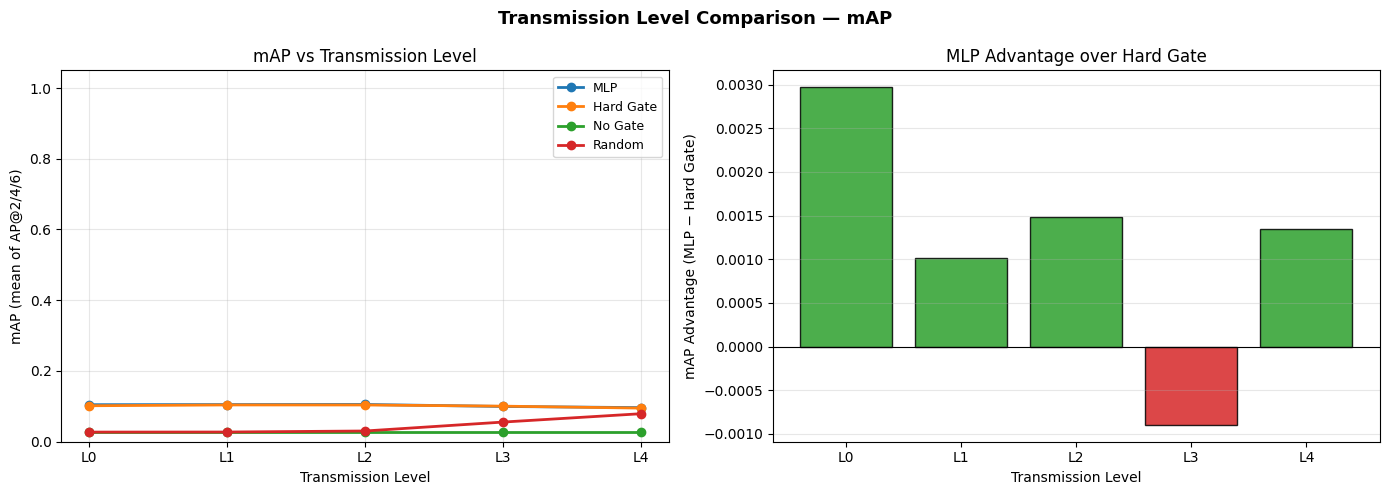
\includegraphics[width=\textwidth]{transmission_level_comparison_mAP.png}
\caption{mAP vs transmission level (left) and MLP advantage over Hard Gate (right).
         The MLP leads at L0--L2 where the budget is sufficient for selection to matter.
         At L3--L4 the gap falls within sampling noise ($N_{\max} \leq 4$ objects per
         frame), and at L4 the Random baseline closes in as forced randomness
         occasionally selects high-value candidates.}
\label{fig:tx_comparison}
\end{figure}

\subsubsection{Limitations}

\paragraph{Dataset scale and label sparsity.}
Only 98 of 462 frames with blind spot candidates provided usable ground-truth supervision, yielding 348 positive object-level labels from 14{,}644 total candidates (2.4\% positive rate). The model is trained on these object-level labels directly, so the supervision signal is sparser than the frame count alone suggests. The class imbalance is handled by positive-class weighting ($w_+ = 51.5$), but with this few positives the MLP cannot be expected to generalize well to scene types not represented in the training set.

\paragraph{BEV localization error.}
The mean BEV localization error of 20.93\,m against the cooperative ground truth is large relative to the 2--6\,m AP thresholds used in evaluation, directly suppressing AP@2m across all strategies. The primary source is the size-prior monocular depth estimator $Z = f_y H_{\text{real}} / H_{\text{pixel}}$, which degrades beyond approximately 60\,m where objects span only a few pixel rows. A learned metric depth network or stereo camera setup would substantially reduce this error.

\paragraph{Temporal consistency.}
The pipeline operates frame-by-frame. A Kalman filter or similar state estimator applied to world-coordinate tracks would smooth positional estimates over time and reduce the effect of single-frame outliers on the blind spot detection decision, as well as increasing the number of usable positive labels for training.

\paragraph{Coordinate alignment.}
The DAIR-V2X system error offset $(\Delta x, \Delta y)$ corrects for a static positioning bias between the infrastructure and vehicle world frames. The high exclusion rate (364 of 462 frames) suggests misalignment beyond what this offset can correct, possibly due to calibration noise, temporal mismatch between frame pairs, or accumulated projection error. Real deployments would require an online relative pose estimation step to handle dynamic GPS drift and multipath interference.

\paragraph{Channel model fidelity.}
The simulator reports 100\% LOS and a mean ego-RSU distance of 1{,}059.6\,m, which are unrealistic for an intersection-based RSU. These figures arise because the cooperative frame pairs in DAIR-V2X are matched by sequential index rather than true temporal or spatial synchronization. A properly synchronized deployment would show a realistic LOS/NLOS mixture at shorter operational ranges.

\paragraph{Single infrastructure node.}
The system assumes a single RSU. Extending to multiple RSUs or V2V links would broaden scene coverage but requires multi-source track fusion and consistent ID management across nodes, both of which are non-trivial problems left for future work.

\subsubsection{Future Work}

Replacing the size-prior depth estimator with a metric monocular depth network would directly address the dominant source of localization error and extend reliable BEV estimation to objects at greater range. The Semantic Gate MLP could be extended to a recurrent architecture that conditions selection on a short history of channel states and candidate scores, enabling smoother decisions across frames. Integrating the covariance calibration into an online loop where $k$, $\sigma_{x_0}$, and $k_x$ are updated continuously from confirmed matches would allow the system to adapt to changing conditions without an offline calibration step. Finally, evaluating the full pipeline on a larger cooperative benchmark such as V2X-ViT or OPV2V, which provide more frames and well-registered world frames, would be an important step toward validating the system for real deployment.


\section{Experimental Results}
\label{sec:results}

\subsection{mAP Evaluation Results}

The mAP evaluation measures how accurately the full system identifies and localizes blind spot targets at three distance thresholds: 2m, 4m, and 6m. Four strategies are compared across all thresholds and transmission levels. Figure~\ref{fig:full_eval} shows the complete evaluation dashboard.

\begin{figure}[htbp]
\centering
\includegraphics[width=\textwidth]{full_evaluation.png}
\caption{Full system evaluation. Top row: BEV localization accuracy. Middle rows: blind spot matching statistics, gate score distribution, Precision-Recall curve, and average recall. Bottom row: ablation and AUC scores.}
\label{fig:full_eval}
\end{figure}

\medskip
Across the 2,832 cooperative frame pairs processed, the system identified 14,505 blind spot candidates of which 309 were confirmed true positives. The MLP Semantic Gate achieves a mean recall of 0.588, compared to 0.569 for Hard Gate, 0.131 for No Gate, and roughly 0.057 for Random. The gap between MLP and Hard Gate is modest in absolute terms but consistent and holds across all five transmission levels rather than appearing only under specific conditions. The ROC-AUC of 0.989 confirms the MLP ranks candidates well overall, and the PR-AUC of 0.551 against a random baseline of 0.023 shows that ranking quality translates into real retrieval performance on a heavily imbalanced dataset where true blind spot targets make up only a small fraction of all candidates.

\medskip
Figure~\ref{fig:semantic_eval} breaks recall down by scenario. In Near/LOS conditions the MLP hits 1.00. When targets are close and the channel budget is large enough to transmit all of them, the ranking barely matters. The difference shows up in the Medium and Far/NLOS scenarios, where the budget shrinks and the MLP's ability to rank the right targets to the top of the list starts to matter. At Far/NLOS, MLP recall drops to around 0.68, while Hard Gate falls to roughly 0.42. The gap is largest precisely where it counts most, when targets are hardest to detect and the channel is tightest.

\begin{figure}[htbp]
\centering
\includegraphics[width=\textwidth]{semantic_gate_eval.png}
\caption{Blind spot recall by strategy and scenario. Error bars show standard deviation across channel budget samples.}
\label{fig:semantic_eval}
\end{figure}

\medskip
At the tightest bandwidth level, L4 (204,800 bytes per target), the budget shrinks to just 3--4 targets per frame and all strategies converge. When only three objects can be sent, there is little room for a learned ranking to show its advantage over a heuristic one. This is an expected limitation of the setup rather than a failure of the model, under extreme bandwidth constraints, any reasonable selection policy will perform similarly.

\section{Conclusion and Future Work}
\label{sec:conclusion}

\printbibliography[title={References}]

\end{document}